\chapter{The Static Universe: Quantum Cosmology}
\label{chap:wdw}

\section{Everett without Branching}

We have landed in static fully self contained universe which just is. Every possible state of every possible system is already ``compiled" into a single, massive, static lookup table.

This is the Wheeler-DeWitt (WdW) universe. Standard physics often interprets this via the many-worlds (Everettian) view, but with a branching mechanism.
In our informational framework, we refuse to rely on metaphysical branching. There is only a static configuration space $\mathcal{C}$ of $2^n$ bits. Every "Everettian world" is simply a different
configuration in this massive set of information.

The question then is: if everything exists at once, why do we experience a sequential "now"?
As demonstrated earlier, the answer is that we find ourselves along the observer-compatible histories occupying the largest low-complexity equivalence classes.


\section{Quantum Cosmology: Spectral Complexity and the Measure of Observers}

To formalize this, we apply our theory to the scale of the entire cosmos.
In standard quantum cosmology, physicists use a "Wick rotation" to imaginary time to make their math work. 
Rather than relying on Euclidean continuation, we introduce an alternative informational weighting principle based on spectral complexity.


\subsection*{Introduction}

The canonical quantization of general relativity leads to the Wheeler-DeWitt equation \cite{dewitt1967}:
\begin{equation}
\hat{\mathcal{H}} \Psi[g_{ij}, \phi] = 0,
\end{equation}
where $\Psi$ is the wavefunction of the universe. This equation is timeless. The ``Problem of Time'' arises because all physical predictions must be extracted from a single, static superposition.

In this work, we propose \textit{Spectral Quantum Cosmology} (SQC).
We remain strictly within the static WdW framework and introduce an information-theoretic selection principle based on \textit{Spectral Complexity}.
Rather than weighting geometries via Euclidean action, we weight possible \textit{observer wavefunctions} directly.
Observers with simpler internal descriptions dominate the measure.

\section{Relational Observers in a Timeless Universe}

Following Page and Wootters \cite{page1983clock}, time emerges relationally.
The universal wavefunction $\Psi$ is static and contains entangled subsystems: a clock degree of freedom and the rest of the universe.

An observer corresponds to a wavefunction $\psi_o$ that is entangled with a suitable clock variable $\lambda$ (like the scale factor of the universe).
The experienced flow of time arises from correlations between observer states and relational clock degrees of freedom within the static universal wavefunction.

\section{Spectral Complexity as the Measure}

As derived in the Chapter~\nameref{chap:framework-of-everything} we define the \textit{Spectral Complexity} of an observer wavefunction $\psi_o(\lambda)$ as the minimal information cost of representing it in the frequency domain.

Observers requiring highly oscillatory or spectrally incoherent descriptions are exponentially suppressed.
Conversely, observers who experience smooth, law-like evolution dominate the measure.
This replaces the "imaginary time" trick of standard physics with a native algorithmic measure.


\section{Testing the Idea in a Simple Simulation}

We implemented a minimal simulation (2 spatial and 1 time dimension) to see if our "Minimal Complexity" path matched the "Least Action" path of traditional physics.

\begin{figure}[h]
\centering
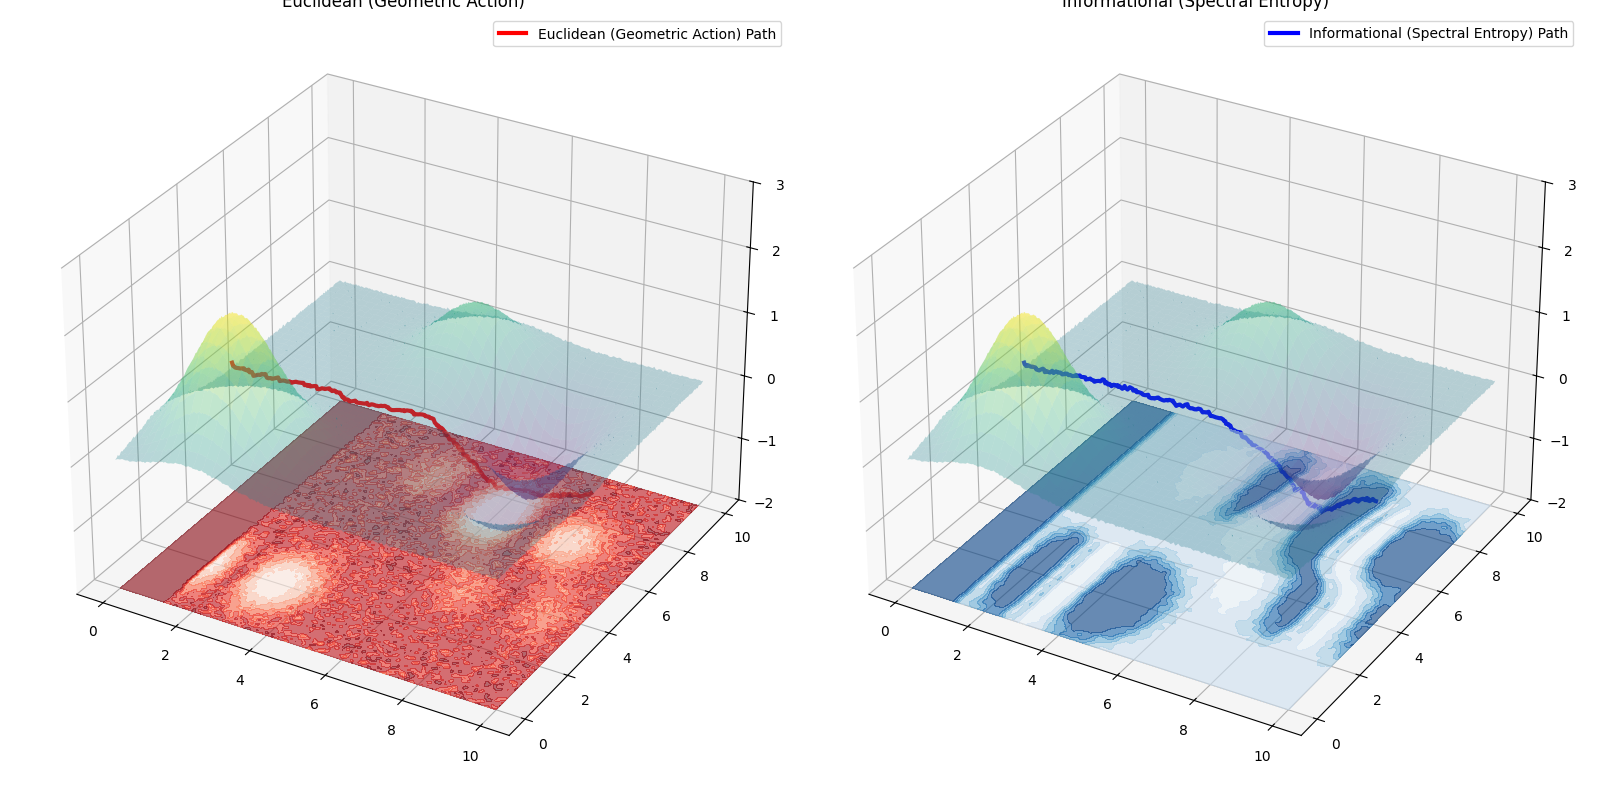
\includegraphics[width=0.8\textwidth]{figures/wdwfields.png}
\caption{Side-by-side comparison: The classical field (Euclidean Action) vs.
  The Informational field (Induced Measure). Preliminary numerical results indicate rough agreement between minimal spectral complexity trajectories and classical least-action solutions.}
\end{figure}


\begin{figure}[h]
\centering
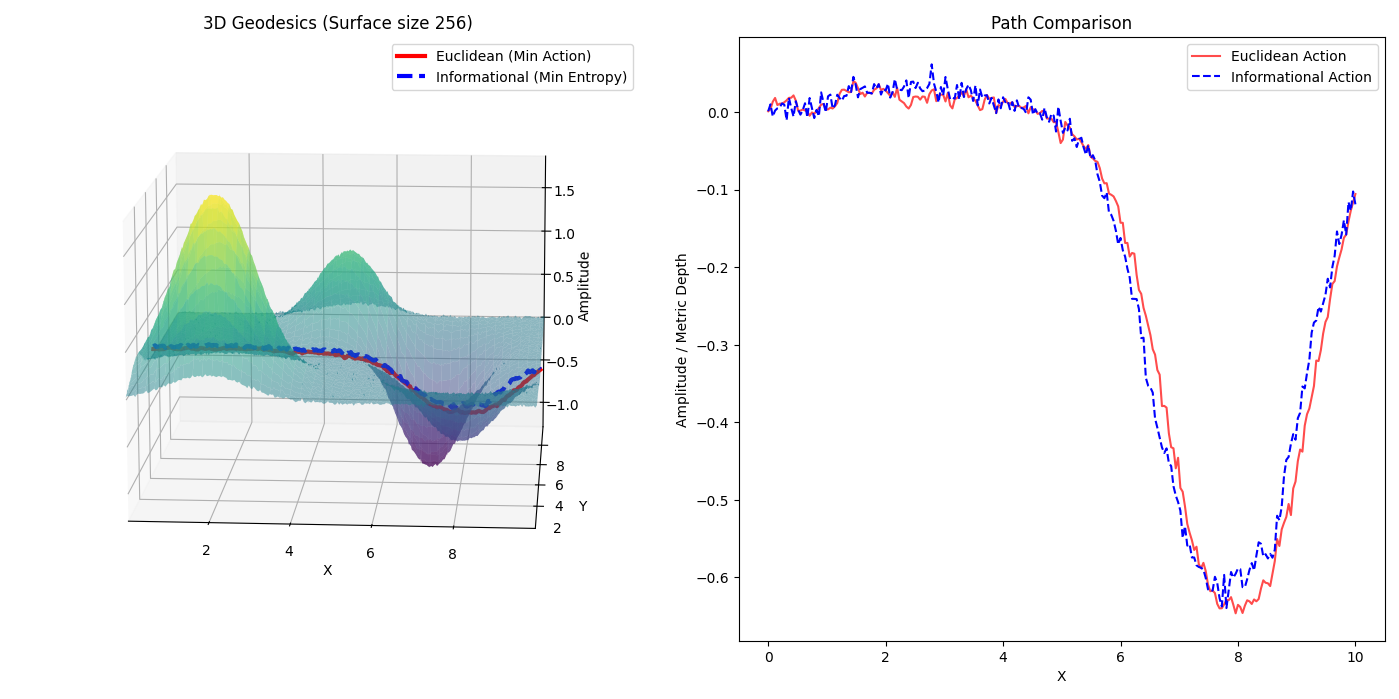
\includegraphics[width=0.8\textwidth]{figures/wdwpaths.png}
\caption{Side-by-side comparison: The classical path (Euclidean Action) vs.
  The Informational path (Induced Measure). Preliminary numerical results indicate strong qualitative agreement between minimal spectral complexity trajectories and classical least-action solutions.}
\end{figure}


The results were promising. 
The path that is "simplest to describe" spectrally matches approximately the path that Einstein’s equations predict.
The apparent fuzziness of microscopic physics may reflect limitations inherent in finite observer-side spectral representation.

\section{Conclusion}

When applied to cosmology, the framework naturally converges toward an effective Wheeler--DeWitt description:
a timeless, self-contained universe in which dynamics emerge relationally through observer-conditioned correlations.


\section{Future Work}

The simulations were 2D toy-models with predefined metric without backreaction.
Implement a true closed FLRW minisuperspace simulation.
